\documentclass{article}
\usepackage{hyperref}
\usepackage{graphics}
\title{Laboratory automation in a functional programming language}
\author{C. Runciman \and A. Clare \and R. Harkness}
\date{Published in Journal of Laboratory Automation\\2014 Dec; 19(6):569-76. doi: 10.1177/2211068214543373.\\ \url{http://jla.sagepub.com/content/19/6/569.abstract}}
%% ODER: format ==         = "\mathrel{==}"
%% ODER: format /=         = "\neq "
%
%
\makeatletter
\@ifundefined{lhs2tex.lhs2tex.sty.read}%
  {\@namedef{lhs2tex.lhs2tex.sty.read}{}%
   \newcommand\SkipToFmtEnd{}%
   \newcommand\EndFmtInput{}%
   \long\def\SkipToFmtEnd#1\EndFmtInput{}%
  }\SkipToFmtEnd

\newcommand\ReadOnlyOnce[1]{\@ifundefined{#1}{\@namedef{#1}{}}\SkipToFmtEnd}
\usepackage{amstext}
\usepackage{amssymb}
\usepackage{stmaryrd}
\DeclareFontFamily{OT1}{cmtex}{}
\DeclareFontShape{OT1}{cmtex}{m}{n}
  {<5><6><7><8>cmtex8
   <9>cmtex9
   <10><10.95><12><14.4><17.28><20.74><24.88>cmtex10}{}
\DeclareFontShape{OT1}{cmtex}{m}{it}
  {<-> ssub * cmtt/m/it}{}
\newcommand{\texfamily}{\fontfamily{cmtex}\selectfont}
\DeclareFontShape{OT1}{cmtt}{bx}{n}
  {<5><6><7><8>cmtt8
   <9>cmbtt9
   <10><10.95><12><14.4><17.28><20.74><24.88>cmbtt10}{}
\DeclareFontShape{OT1}{cmtex}{bx}{n}
  {<-> ssub * cmtt/bx/n}{}
\newcommand{\tex}[1]{\text{\texfamily#1}}	% NEU

\newcommand{\Sp}{\hskip.33334em\relax}


\newcommand{\Conid}[1]{\mathit{#1}}
\newcommand{\Varid}[1]{\mathit{#1}}
\newcommand{\anonymous}{\kern0.06em \vbox{\hrule\@width.5em}}
\newcommand{\plus}{\mathbin{+\!\!\!+}}
\newcommand{\bind}{\mathbin{>\!\!\!>\mkern-6.7mu=}}
\newcommand{\rbind}{\mathbin{=\mkern-6.7mu<\!\!\!<}}% suggested by Neil Mitchell
\newcommand{\sequ}{\mathbin{>\!\!\!>}}
\renewcommand{\leq}{\leqslant}
\renewcommand{\geq}{\geqslant}
\usepackage{polytable}

%mathindent has to be defined
\@ifundefined{mathindent}%
  {\newdimen\mathindent\mathindent\leftmargini}%
  {}%

\def\resethooks{%
  \global\let\SaveRestoreHook\empty
  \global\let\ColumnHook\empty}
\newcommand*{\savecolumns}[1][default]%
  {\g@addto@macro\SaveRestoreHook{\savecolumns[#1]}}
\newcommand*{\restorecolumns}[1][default]%
  {\g@addto@macro\SaveRestoreHook{\restorecolumns[#1]}}
\newcommand*{\aligncolumn}[2]%
  {\g@addto@macro\ColumnHook{\column{#1}{#2}}}

\resethooks

\newcommand{\onelinecommentchars}{\quad-{}- }
\newcommand{\commentbeginchars}{\enskip\{-}
\newcommand{\commentendchars}{-\}\enskip}

\newcommand{\visiblecomments}{%
  \let\onelinecomment=\onelinecommentchars
  \let\commentbegin=\commentbeginchars
  \let\commentend=\commentendchars}

\newcommand{\invisiblecomments}{%
  \let\onelinecomment=\empty
  \let\commentbegin=\empty
  \let\commentend=\empty}

\visiblecomments

\newlength{\blanklineskip}
\setlength{\blanklineskip}{0.66084ex}

\newcommand{\hsindent}[1]{\quad}% default is fixed indentation
\let\hspre\empty
\let\hspost\empty
\newcommand{\NB}{\textbf{NB}}
\newcommand{\Todo}[1]{$\langle$\textbf{To do:}~#1$\rangle$}

\EndFmtInput
\makeatother
%
%
%
%
%
%
% This package provides two environments suitable to take the place
% of hscode, called "plainhscode" and "arrayhscode". 
%
% The plain environment surrounds each code block by vertical space,
% and it uses \abovedisplayskip and \belowdisplayskip to get spacing
% similar to formulas. Note that if these dimensions are changed,
% the spacing around displayed math formulas changes as well.
% All code is indented using \leftskip.
%
% Changed 19.08.2004 to reflect changes in colorcode. Should work with
% CodeGroup.sty.
%
\ReadOnlyOnce{polycode.fmt}%
\makeatletter

\newcommand{\hsnewpar}[1]%
  {{\parskip=0pt\parindent=0pt\par\vskip #1\noindent}}

% can be used, for instance, to redefine the code size, by setting the
% command to \small or something alike
\newcommand{\hscodestyle}{}

% The command \sethscode can be used to switch the code formatting
% behaviour by mapping the hscode environment in the subst directive
% to a new LaTeX environment.

\newcommand{\sethscode}[1]%
  {\expandafter\let\expandafter\hscode\csname #1\endcsname
   \expandafter\let\expandafter\endhscode\csname end#1\endcsname}

% "compatibility" mode restores the non-polycode.fmt layout.

\newenvironment{compathscode}%
  {\par\noindent
   \advance\leftskip\mathindent
   \hscodestyle
   \let\\=\@normalcr
   \let\hspre\(\let\hspost\)%
   \pboxed}%
  {\endpboxed\)%
   \par\noindent
   \ignorespacesafterend}

\newcommand{\compaths}{\sethscode{compathscode}}

% "plain" mode is the proposed default.
% It should now work with \centering.
% This required some changes. The old version
% is still available for reference as oldplainhscode.

\newenvironment{plainhscode}%
  {\hsnewpar\abovedisplayskip
   \advance\leftskip\mathindent
   \hscodestyle
   \let\hspre\(\let\hspost\)%
   \pboxed}%
  {\endpboxed%
   \hsnewpar\belowdisplayskip
   \ignorespacesafterend}

\newenvironment{oldplainhscode}%
  {\hsnewpar\abovedisplayskip
   \advance\leftskip\mathindent
   \hscodestyle
   \let\\=\@normalcr
   \(\pboxed}%
  {\endpboxed\)%
   \hsnewpar\belowdisplayskip
   \ignorespacesafterend}

% Here, we make plainhscode the default environment.

\newcommand{\plainhs}{\sethscode{plainhscode}}
\newcommand{\oldplainhs}{\sethscode{oldplainhscode}}
\plainhs

% The arrayhscode is like plain, but makes use of polytable's
% parray environment which disallows page breaks in code blocks.

\newenvironment{arrayhscode}%
  {\hsnewpar\abovedisplayskip
   \advance\leftskip\mathindent
   \hscodestyle
   \let\\=\@normalcr
   \(\parray}%
  {\endparray\)%
   \hsnewpar\belowdisplayskip
   \ignorespacesafterend}

\newcommand{\arrayhs}{\sethscode{arrayhscode}}

% The mathhscode environment also makes use of polytable's parray 
% environment. It is supposed to be used only inside math mode 
% (I used it to typeset the type rules in my thesis).

\newenvironment{mathhscode}%
  {\parray}{\endparray}

\newcommand{\mathhs}{\sethscode{mathhscode}}

% texths is similar to mathhs, but works in text mode.

\newenvironment{texthscode}%
  {\(\parray}{\endparray\)}

\newcommand{\texths}{\sethscode{texthscode}}

% The framed environment places code in a framed box.

\def\codeframewidth{\arrayrulewidth}
\RequirePackage{calc}

\newenvironment{framedhscode}%
  {\parskip=\abovedisplayskip\par\noindent
   \hscodestyle
   \arrayrulewidth=\codeframewidth
   \tabular{@{}|p{\linewidth-2\arraycolsep-2\arrayrulewidth-2pt}|@{}}%
   \hline\framedhslinecorrect\\{-1.5ex}%
   \let\endoflinesave=\\
   \let\\=\@normalcr
   \(\pboxed}%
  {\endpboxed\)%
   \framedhslinecorrect\endoflinesave{.5ex}\hline
   \endtabular
   \parskip=\belowdisplayskip\par\noindent
   \ignorespacesafterend}

\newcommand{\framedhslinecorrect}[2]%
  {#1[#2]}

\newcommand{\framedhs}{\sethscode{framedhscode}}

% The inlinehscode environment is an experimental environment
% that can be used to typeset displayed code inline.

\newenvironment{inlinehscode}%
  {\(\def\column##1##2{}%
   \let\>\undefined\let\<\undefined\let\\\undefined
   \newcommand\>[1][]{}\newcommand\<[1][]{}\newcommand\\[1][]{}%
   \def\fromto##1##2##3{##3}%
   \def\nextline{}}{\) }%

\newcommand{\inlinehs}{\sethscode{inlinehscode}}

% The joincode environment is a separate environment that
% can be used to surround and thereby connect multiple code
% blocks.

\newenvironment{joincode}%
  {\let\orighscode=\hscode
   \let\origendhscode=\endhscode
   \def\endhscode{\def\hscode{\endgroup\def\@currenvir{hscode}\\}\begingroup}
   %\let\SaveRestoreHook=\empty
   %\let\ColumnHook=\empty
   %\let\resethooks=\empty
   \orighscode\def\hscode{\endgroup\def\@currenvir{hscode}}}%
  {\origendhscode
   \global\let\hscode=\orighscode
   \global\let\endhscode=\origendhscode}%

\makeatother
\EndFmtInput
%
\begin{document}
\maketitle


\begin{abstract}
After some years of use in academic and research settings, functional languages are starting to enter the mainstream as an alternative to more conventional programming languages. This article explores one way to use Haskell, a functional programming language, in the development of control programs for laboratory automation systems. We give code for an example system, discuss some programming concepts that we need for this example, and demonstrate how the use of functional programming allows us to express and verify properties of the resulting code.
\end{abstract}

\section{Introduction}

There are many different types of software applications in the field of laboratory automation.  There are stand-alone applications for controlling a simple instrument such as a bulk-reagent dispenser. There are also larger software packages for controlling automated robotic systems with many instruments that are linked to data management systems [1]. These software packages are typically referred to as schedulers.

Currently, popular languages for laboratory-automation applications include Java, C, C++ and C\#. In our experience, the majority of such applications have been developed using these languages, along with other .NET variants such as Visual Basic.NET [2].  

These languages are commonly known as procedural or imperative languages. They describe the commands to use in a sequential manner, to achieve the intended functionality. They change state, such as the value of variables, along the way and the values of these variables can dictate the flow of execution.  Although languages such as Java and C++ use different syntax, the general principles of constructing code remain the same.

An imperative approach is the most common way to develop an application. There are though, different programming styles that can be adopted, one of these being the functional approach.  Functional languages, such as O'Caml and Haskell are not as well-known as C or C\#, especially among programmers from a non-computer science background.  However, since Microsoft released Visual Studio 2010 with the inclusion of F\# and the increased adoption of Scala, there has been an increasing awareness of functional languages among commercial application developers.  Originally a research project at Microsoft that based itself upon O’Caml, F\# has developed into a functional language that interacts with the Microsoft .NET library [3]. Indeed, anyone who has used the .NET Framework 3.5 is quite likely to be familiar with some functional language concepts without realizing it.  For example, the design of LINQ queries within the .NET Framework was based upon the use of anonymous functions within Haskell.

The remainder of this article provides a complete and executable program that implements a scheduler for laboratory automation. Along the way, we gently introduce the Haskell programming language and point out the properties that are declared in the code. We start by defining types, move on to define auxiliary functions, build up the scheduler, and finish with a section on automated testing of properties of interest.


\subsection*{The Scheduling Problem}

Scheduling is an important component of a laboratory automation software package [4,5].  The benefit of using laboratory automation is that multiple plates within an experiment or assay can be processed automatically.  To improve efficiency, the schedule must allow multiple plates to run at the same time so the execution is interleaved, which then maximizes throughput.  

One simple approach is to use an event-driven scheduling system. This works by assessing the state of the system on a continual cycle. After each event, the scheduler, or processing engine, determines a course of action for the system to run as quickly as possible without breaking constraints such as incubation times and the maximum number of plates allowed on each device. For example, if a plate is due out of an incubator, this task is given priority over adding a new plate into the system. The advantage of an event-driven system is that the assay can follow different processing paths based upon events, such as acquired data or the failure of an instrument in the system.

However, with an event driven scheduler, there is the possibility of encountering scheduling deadlocks. A simple example of a deadlock is where:
\begin{itemize}
\item Plate 1, sitting on Instrument A needs to move to Instrument B and 
\item Plate 2, sitting on Instrument B wants to move to Instrument A.
\end{itemize} 

It is not possible for either plate to move onto the next step within its respective workflow, so there is deadlock. Deadlock situations can involve more plates and instruments, but the basic problem is the same: it is not possible to unblock key resources to allow the workflow for each plate to be processed.

In the remainder of this article we illustrate the use of functional programming as a style of programming that can help in defining control software for laboratory automation. This will bring out many of the distinctive aspects of functional programming as we develop the code. In order to make this illustration we use a particular hardware setup that can be found in many laboratories. The system has an input stack, an output stack, and some number of washers and dispensers, as shown in Figure \ref{fig:system}.

\begin{figure}
\scalebox{0.8}{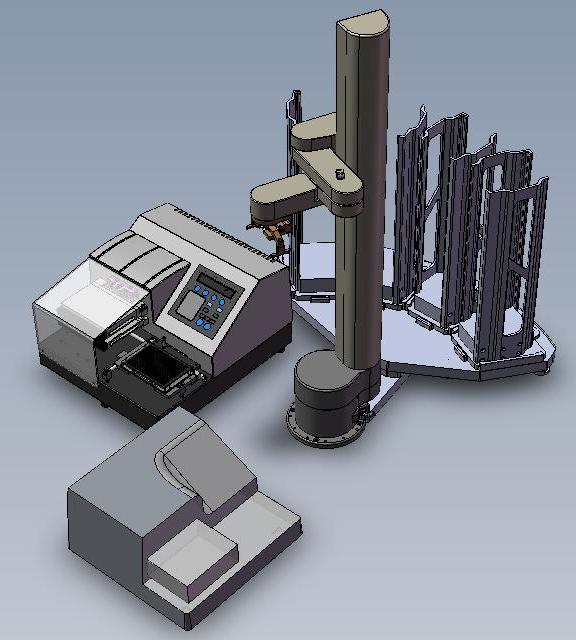
\includegraphics{system.png}}
\caption{An example system with input stack, output stack, robot arm, washer, and dispenser. This is the simplest type of automated platform whereby more than one plate will be active on the system at the same time. With this platform, an optimal schedule will have the washer and the dispenser occupied simultaneously.}
\label{fig:system}
\end{figure}

Here are some of the properties we want our laboratory scheduler to have:
\begin{enumerate}
\item each plate has a workflow;
\item each device, including the robot, requires a specified period of time to do its job;
\item each plate progresses through its workflow in a timely manner;
\item the whole system is deadlock-free.
\end{enumerate}

Using a functional programming language allows us to write in a style that can express and verify such properties rather than just write code. Properties 1 and 2 can be expressed in types for plates and devices, statically checked by a compiler.  Properties 3 and 4 can be expressed in property functions and checked by property-based testing tools such as QuickCheck [6] or SmallCheck [7]. 

By formulating properties in this way, developers can capture general rules about the required behaviour of a system, not just specific cases and fragments represented by unit tests. Computing power is harnessed to search the space of possible test inputs automatically, looking for cases in which one of the specified properties fails. The technique is also known as ``lightweight verification'' as it is the next best thing to a rigorous mathematical verification that all the formulated properties hold in all cases.


\section{Method and Results}

\subsection*{Devices and Workflows}

We begin with some import statements allowing us to use standard library functions.
\begin{hscode}\SaveRestoreHook
\column{B}{@{}>{\hspre}l<{\hspost}@{}}%
\column{3}{@{}>{\hspre}l<{\hspost}@{}}%
\column{E}{@{}>{\hspre}l<{\hspost}@{}}%
\>[3]{}\mathbf{import}\;\Conid{\Conid{Data}.List}\;((\mathbin{\char92 \char92 }),\Varid{union}){}\<[E]%
\\
\>[3]{}\mathbf{import}\;\Conid{\Conid{Test}.QuickCheck}{}\<[E]%
\ColumnHook
\end{hscode}\resethooks
First we must choose how to represent the kinds of devices found in a laboratory, such as washer and dispenser. This choice is reflected in the definition of our first datatype. 

One can think of a type as a description of a set of possible values, or equivalently a type is a property that any value may or may not have. Our first type is \text{\tt DeviceKind}. It has four possible values for the four kinds of devices in our laboratory. Only these values have the property that they are of type \text{\tt DeviceKind}. 

\begin{hscode}\SaveRestoreHook
\column{B}{@{}>{\hspre}l<{\hspost}@{}}%
\column{3}{@{}>{\hspre}l<{\hspost}@{}}%
\column{54}{@{}>{\hspre}l<{\hspost}@{}}%
\column{E}{@{}>{\hspre}l<{\hspost}@{}}%
\>[3]{}\mathbf{data}\;\Conid{DeviceKind}\mathrel{=}\Conid{Washer}\mid \Conid{Dispenser}\mid \Conid{InStack}\mid \Conid{OutStack}{}\<[E]%
\\
\>[3]{}\hsindent{51}{}\<[54]%
\>[54]{}\mathbf{deriving}\;(\Conid{Eq},\Conid{Show}){}\<[E]%
\ColumnHook
\end{hscode}\resethooks
Informally the vertical bar can be read ``or'': so a value of type \text{\tt DeviceKind} is a \text{\tt Washer} or a \text{\tt Dispenser} or an \text{\tt InStack} or an \text{\tt OutStack}.

The deriving clause gives us two properties of the \text{\tt DeviceKind} type: it belongs to the type-class \text{\tt Eq} (so its values can be compared for equality) and it belongs to the type-class \text{\tt Show} (so its values can be printed as strings).  A type-class is similar to an interface in Java or C\#, for which we must provide implementations of functions. In using the keyword ``\text{\tt deriving}'' we accept the default implementations for this type. 

With the \text{\tt DeviceKind} type defined, one simple representation of a laboratory workflow, sufficient for the purposes of this article, is a list of devices that a microtitre plate must go to in turn. Lists are a built-in datatype in Haskell. The way that lists are defined guarantees that items in the same list are of the same type. 
\begin{hscode}\SaveRestoreHook
\column{B}{@{}>{\hspre}l<{\hspost}@{}}%
\column{3}{@{}>{\hspre}l<{\hspost}@{}}%
\column{E}{@{}>{\hspre}l<{\hspost}@{}}%
\>[3]{}\mathbf{type}\;\Conid{Workflow}\mathrel{=}[\mskip1.5mu \Conid{DeviceKind}\mskip1.5mu]{}\<[E]%
\ColumnHook
\end{hscode}\resethooks
Here \text{\tt Workflow} is defined as a synonym for a list of \text{\tt DeviceKind}. We define the following example workflow for use in later tests.
\begin{hscode}\SaveRestoreHook
\column{B}{@{}>{\hspre}l<{\hspost}@{}}%
\column{3}{@{}>{\hspre}l<{\hspost}@{}}%
\column{E}{@{}>{\hspre}l<{\hspost}@{}}%
\>[3]{}\Varid{exampleWorkflow}\mathbin{::}\Conid{Workflow}{}\<[E]%
\\
\>[3]{}\Varid{exampleWorkflow}\mathrel{=}[\mskip1.5mu \Conid{InStack},\Conid{Washer},\Conid{Dispenser},\Conid{Washer},\Conid{OutStack}\mskip1.5mu]{}\<[E]%
\ColumnHook
\end{hscode}\resethooks
One simple but useful function on lists is \text{\tt null}, which tests its list argument for emptiness.  Here’s how we can use it to define \text{\tt nonEmpty}, a function that tests for a non-empty list.
\begin{hscode}\SaveRestoreHook
\column{B}{@{}>{\hspre}l<{\hspost}@{}}%
\column{3}{@{}>{\hspre}l<{\hspost}@{}}%
\column{E}{@{}>{\hspre}l<{\hspost}@{}}%
\>[3]{}\Varid{nonEmpty}\;\Varid{xs}\mathrel{=}\neg \;(\Varid{null}\;\Varid{xs}){}\<[E]%
\ColumnHook
\end{hscode}\resethooks
Function applications are frequent in functional programs so the notation needs to be light.  In Haskell, we just write a function name then each of the input arguments in turn.  No extra symbols such as brackets or commas are needed.  The brackets in \text{\tt not~\char40{}null~xs\char41{}} merely indicate priority: without them, \text{\tt not~null~xs} would apply the function \text{\tt not} to the two arguments \text{\tt null} and \text{\tt xs}.

We shall often make use of the infix colon operator for constructing non-empty lists. The list \text{\tt e\char58{}rest} contains a first element \text{\tt e}, followed by a (possibly empty) list `\text{\tt rest}' of other elements.

We need some representation of time. For example, we must represent the time needed for processing by each device and for transfer of plates between devices. For the purposes of this article a time value is simply an integer representing a number of ``ticks''. Whether ticks are milliseconds, seconds or something else need not concern us.
\begin{hscode}\SaveRestoreHook
\column{B}{@{}>{\hspre}l<{\hspost}@{}}%
\column{3}{@{}>{\hspre}l<{\hspost}@{}}%
\column{E}{@{}>{\hspre}l<{\hspost}@{}}%
\>[3]{}\mathbf{type}\;\Conid{Time}\mathrel{=}\Conid{Int}{}\<[E]%
\ColumnHook
\end{hscode}\resethooks
There may be more than one device in the lab of the same kind (for example we may have two washers). So we also define a further type whose values represent specific devices. A specific \text{\tt Device} is represented by a combination of a \text{\tt DeviceKind} value, an integer to distinguish this device from others of the same kind, the length of time for this device to process a plate and the length of time for a robot arm to move a plate between this device and a central safe location. For example if we have two washers in our system, they might be represented by the values \text{\tt Device~Washer~1~3~2} and \text{\tt Device~Washer~2~3~3}.
\begin{hscode}\SaveRestoreHook
\column{B}{@{}>{\hspre}l<{\hspost}@{}}%
\column{3}{@{}>{\hspre}l<{\hspost}@{}}%
\column{27}{@{}>{\hspre}l<{\hspost}@{}}%
\column{33}{@{}>{\hspre}l<{\hspost}@{}}%
\column{37}{@{}>{\hspre}l<{\hspost}@{}}%
\column{E}{@{}>{\hspre}l<{\hspost}@{}}%
\>[3]{}\mathbf{data}\;\Conid{Device}\mathrel{=}\Conid{Device}\;\{\mskip1.5mu {}\<[27]%
\>[27]{}\Varid{devKind}{}\<[37]%
\>[37]{}\mathbin{::}\Conid{DeviceKind},{}\<[E]%
\\
\>[27]{}\Varid{devNo}{}\<[37]%
\>[37]{}\mathbin{::}\Conid{Int},{}\<[E]%
\\
\>[27]{}\Varid{devProcT}{}\<[37]%
\>[37]{}\mathbin{::}\Conid{Time},{}\<[E]%
\\
\>[27]{}\Varid{devMoveT}{}\<[37]%
\>[37]{}\mathbin{::}\Conid{Time}\mskip1.5mu\}{}\<[E]%
\\
\>[27]{}\hsindent{6}{}\<[33]%
\>[33]{}\mathbf{deriving}\;\Conid{Eq}{}\<[E]%
\ColumnHook
\end{hscode}\resethooks
The above definition describes the fields of a \text{\tt Device}, giving them names and types. It also provides automatic field accessor functions which can be used to inspect the values or provide new values for the fields. As an example the \text{\tt devProcT} for a device \text{\tt d} could be accessed with the expression \text{\tt devProcT~d} and a copy of a device \text{\tt d} with a new \text{\tt devNo} could be created by \text{\tt d\char39{}~\char61{}~d~\char123{}devNo~\char61{}~4\char125{}}.

Rather than deriving an automated default for the printing of \text{\tt Device} values (which would render them as eg \text{\tt \char34{}Device~Washer~6~3~2\char34{}}) we define our own custom instance, omitting the constructor name \text{\tt Device} and also the timing details. 
\begin{hscode}\SaveRestoreHook
\column{B}{@{}>{\hspre}l<{\hspost}@{}}%
\column{3}{@{}>{\hspre}l<{\hspost}@{}}%
\column{5}{@{}>{\hspre}l<{\hspost}@{}}%
\column{28}{@{}>{\hspre}c<{\hspost}@{}}%
\column{28E}{@{}l@{}}%
\column{31}{@{}>{\hspre}l<{\hspost}@{}}%
\column{E}{@{}>{\hspre}l<{\hspost}@{}}%
\>[3]{}\mathbf{instance}\;\Conid{Show}\;\Conid{Device}\;\mathbf{where}{}\<[E]%
\\
\>[3]{}\hsindent{2}{}\<[5]%
\>[5]{}\Varid{show}\;(\Conid{Device}\;\Varid{d}\;\Varid{n}\;\Varid{p}\;\Varid{m}){}\<[28]%
\>[28]{}\mathrel{=}{}\<[28E]%
\>[31]{}\Varid{show}\;\Varid{d}\plus \text{\tt \char34 ~\char34}\plus \Varid{show}\;\Varid{n}{}\<[E]%
\ColumnHook
\end{hscode}\resethooks
When we come to define scheduling, the workflow just specifies a \text{\tt DeviceKind} but the scheduler must allocate a specific \text{\tt Device}. We capture the \text{\tt isA} relationship between devices and device-kinds in the following definition.
\begin{hscode}\SaveRestoreHook
\column{B}{@{}>{\hspre}l<{\hspost}@{}}%
\column{3}{@{}>{\hspre}l<{\hspost}@{}}%
\column{29}{@{}>{\hspre}c<{\hspost}@{}}%
\column{29E}{@{}l@{}}%
\column{33}{@{}>{\hspre}l<{\hspost}@{}}%
\column{E}{@{}>{\hspre}l<{\hspost}@{}}%
\>[3]{}\Varid{isA}\mathbin{::}\Conid{Device}\to \Conid{DeviceKind}\to \Conid{Bool}{}\<[E]%
\\
\>[3]{}\Varid{isA}\;(\Conid{Device}\;\Varid{sd}\;\Varid{n}\;\Varid{p}\;\Varid{m})\;\Varid{d}{}\<[29]%
\>[29]{}\mathrel{=}{}\<[29E]%
\>[33]{}\Varid{sd}==\Varid{d}{}\<[E]%
\ColumnHook
\end{hscode}\resethooks
Functions are values too and they have types. The types declare properties about the function which can be statically checked by the compiler before the program is run. The first line describes the type of this function. The arrows can be read as logical implications. If the first argument is a value of type \text{\tt Device} then if the second is a value of type \text{\tt DeviceKind} then the result is a value of type Bool, a predefined type with the two values \text{\tt True} and \text{\tt False}. Although we can choose to declare the type of a function, in most cases a Haskell compiler can automatically derive this information, so the programmer need not provide it. However, we might choose to provide a type declaration in order to check that our understanding of the function's properties agrees with that derived by the compiler, or just to assist with code readability.

Note that the infix \text{\tt \char61{}\char61{}} is a function that tests values for equality, not to be confused with the single \text{\tt \char61{}} symbol used to define a function. We can also choose to use infix notation when applying named functions: for example, we can write \text{\tt sd~\char96{}isA\char96{}~d} rather than \text{\tt isA~sd~d}, and the infix version makes the roles of \text{\tt sd} and \text{\tt d} clearer.


\subsection*{Plates and Locations}

We are working towards a representation of the complete state of the laboratory. So far we have a representation for devices, but not for the plates that are processed by these devices or for the robot arm that moves plates between them. 

Our next step is to introduce a type to represent the possible locations of plates in the lab. A plate's location is either at a device or it is in transit (by means of the robotic arm) between two devices.  Rather than a long-winded constructor name such as \text{\tt InTransitByRoboticArm}, an infix constructor \text{\tt \char58{}\char45{}\char62{}} gives us a more convenient notation and makes the source and destination clearer. 
\begin{hscode}\SaveRestoreHook
\column{B}{@{}>{\hspre}l<{\hspost}@{}}%
\column{3}{@{}>{\hspre}l<{\hspost}@{}}%
\column{E}{@{}>{\hspre}l<{\hspost}@{}}%
\>[3]{}\mathbf{data}\;\Conid{Loc}\mathrel{=}\Conid{At}\;\Conid{Device}\mid \Conid{Device}\mathbin{:->}\Conid{Device}\;\mathbf{deriving}\;(\Conid{Eq},\Conid{Show}){}\<[E]%
\ColumnHook
\end{hscode}\resethooks
Example \text{\tt Loc} values in their printed form include \text{\tt At~Washer~3} and \text{\tt Washer~3~\char58{}\char45{}\char62{}~Dispenser~1}.

Now we can define the datatype for Plates. 
\begin{hscode}\SaveRestoreHook
\column{B}{@{}>{\hspre}l<{\hspost}@{}}%
\column{3}{@{}>{\hspre}l<{\hspost}@{}}%
\column{25}{@{}>{\hspre}l<{\hspost}@{}}%
\column{27}{@{}>{\hspre}l<{\hspost}@{}}%
\column{37}{@{}>{\hspre}l<{\hspost}@{}}%
\column{E}{@{}>{\hspre}l<{\hspost}@{}}%
\>[3]{}\mathbf{data}\;\Conid{Plate}\mathrel{=}\Conid{Plate}\;\{\mskip1.5mu {}\<[25]%
\>[25]{}\Varid{plateNo}{}\<[37]%
\>[37]{}\mathbin{::}\Conid{Int},{}\<[E]%
\\
\>[25]{}\Varid{plateLoc}{}\<[37]%
\>[37]{}\mathbin{::}\Conid{Loc},{}\<[E]%
\\
\>[25]{}\Varid{plateSince}{}\<[37]%
\>[37]{}\mathbin{::}\Conid{Time},{}\<[E]%
\\
\>[25]{}\Varid{plateFlow}{}\<[37]%
\>[37]{}\mathbin{::}\Conid{Workflow}\mskip1.5mu\}{}\<[E]%
\\
\>[25]{}\hsindent{2}{}\<[27]%
\>[27]{}\mathbf{deriving}\;(\Conid{Eq}){}\<[E]%
\ColumnHook
\end{hscode}\resethooks
The \text{\tt plateNo} is a number uniquely identifying this plate: each plate is allocated a number as it enters the system.  The \text{\tt plateLoc} specifies the current location.  The \text{\tt plateSince} represents the time at which either the plate arrived (for \text{\tt At} locations) or the transfer began (for \text{\tt \char58{}\char45{}\char62{}} locations). The \text{\tt plateFlow} is the remaining list of the kinds of devices this plate must visit. 

When we show a plate as a string, it is usually more convenient to omit the details of the remaining workflow for the plate.
\begin{hscode}\SaveRestoreHook
\column{B}{@{}>{\hspre}l<{\hspost}@{}}%
\column{3}{@{}>{\hspre}l<{\hspost}@{}}%
\column{5}{@{}>{\hspre}l<{\hspost}@{}}%
\column{7}{@{}>{\hspre}l<{\hspost}@{}}%
\column{E}{@{}>{\hspre}l<{\hspost}@{}}%
\>[3]{}\mathbf{instance}\;\Conid{Show}\;\Conid{Plate}\;\mathbf{where}{}\<[E]%
\\
\>[3]{}\hsindent{2}{}\<[5]%
\>[5]{}\Varid{show}\;(\Conid{Plate}\;\Varid{no}\;\Varid{loc}\;\Varid{since}\;\Varid{w})\mathrel{=}{}\<[E]%
\\
\>[5]{}\hsindent{2}{}\<[7]%
\>[7]{}\text{\tt \char34 plate~\char34}\plus \Varid{show}\;\Varid{no}\plus \text{\tt \char34 ,~\char34}\plus \Varid{show}\;\Varid{loc}\plus \text{\tt \char34 ~since~\char34}\plus \Varid{show}\;\Varid{since}{}\<[E]%
\ColumnHook
\end{hscode}\resethooks
Two simple ``helper'' functions extract information from a \text{\tt Plate} value.
\begin{hscode}\SaveRestoreHook
\column{B}{@{}>{\hspre}l<{\hspost}@{}}%
\column{3}{@{}>{\hspre}l<{\hspost}@{}}%
\column{39}{@{}>{\hspre}l<{\hspost}@{}}%
\column{E}{@{}>{\hspre}l<{\hspost}@{}}%
\>[3]{}\Varid{inTransfer}\mathbin{::}\Conid{Plate}\to \Conid{Bool}{}\<[E]%
\\
\>[3]{}\Varid{inTransfer}\;(\Conid{Plate}\;\anonymous \;(\anonymous \mathbin{:->}\anonymous )\;\anonymous \;\anonymous ){}\<[39]%
\>[39]{}\mathrel{=}\Conid{True}{}\<[E]%
\\
\>[3]{}\Varid{inTransfer}\;\anonymous {}\<[39]%
\>[39]{}\mathrel{=}\Conid{False}{}\<[E]%
\ColumnHook
\end{hscode}\resethooks
\begin{hscode}\SaveRestoreHook
\column{B}{@{}>{\hspre}l<{\hspost}@{}}%
\column{3}{@{}>{\hspre}l<{\hspost}@{}}%
\column{E}{@{}>{\hspre}l<{\hspost}@{}}%
\>[3]{}\Varid{plateDestination}\mathbin{::}\Conid{Plate}\to \Conid{Device}{}\<[E]%
\\
\>[3]{}\Varid{plateDestination}\;(\Conid{Plate}\;\anonymous \;(\anonymous \mathbin{:->}\Varid{d})\;\anonymous \;\anonymous )\mathrel{=}\Varid{d}{}\<[E]%
\ColumnHook
\end{hscode}\resethooks
Notice that we don't have to give names to every component in the \text{\tt Plate} value. When a function does not need to refer to a component, we write \text{\tt \char95{}} in the argument pattern. 

With representation types in hand for devices, time and plates, we can complete the data model for the state of the lab-automation system with the following datatype declaration and associated Show instance.
\begin{hscode}\SaveRestoreHook
\column{B}{@{}>{\hspre}l<{\hspost}@{}}%
\column{3}{@{}>{\hspre}l<{\hspost}@{}}%
\column{5}{@{}>{\hspre}l<{\hspost}@{}}%
\column{31}{@{}>{\hspre}l<{\hspost}@{}}%
\column{42}{@{}>{\hspre}l<{\hspost}@{}}%
\column{E}{@{}>{\hspre}l<{\hspost}@{}}%
\>[3]{}\mathbf{data}\;\Conid{SysState}\mathrel{=}\Conid{SysState}\;\{\mskip1.5mu {}\<[31]%
\>[31]{}\Varid{sysPlates}{}\<[42]%
\>[42]{}\mathbin{::}[\mskip1.5mu \Conid{Plate}\mskip1.5mu],{}\<[E]%
\\
\>[31]{}\Varid{sysDevs}{}\<[42]%
\>[42]{}\mathbin{::}[\mskip1.5mu \Conid{Device}\mskip1.5mu],{}\<[E]%
\\
\>[31]{}\Varid{sysTime}{}\<[42]%
\>[42]{}\mathbin{::}\Conid{Time}\mskip1.5mu\}{}\<[E]%
\\
\>[3]{}\mathbf{instance}\;\Conid{Show}\;\Conid{SysState}\;\mathbf{where}{}\<[E]%
\\
\>[3]{}\hsindent{2}{}\<[5]%
\>[5]{}\Varid{show}\;(\Conid{SysState}\;\Varid{ps}\;\Varid{ds}\;\Varid{t})\mathrel{=}\text{\tt \char34 t~=~\char34}\plus \Varid{show}\;\Varid{t}\plus \text{\tt \char34 :~\char34}\plus \Varid{show}\;\Varid{ps}{}\<[E]%
\ColumnHook
\end{hscode}\resethooks
The time in each \text{\tt SysState} is the time at which that state exists. The plates list represents all the plates in the system at that time, including those in the \text{\tt OutStack} for which the workflow has been completed. The devices list represents every device that is in use or available for use at that time.


\subsection*{Events and Scheduling Definition}

We shall model the laboratory process as an event-driven system.  By now it should be no surprise that we want to introduce a new data type, this time to model the four kinds of event that can occur.
\begin{hscode}\SaveRestoreHook
\column{B}{@{}>{\hspre}l<{\hspost}@{}}%
\column{3}{@{}>{\hspre}l<{\hspost}@{}}%
\column{5}{@{}>{\hspre}l<{\hspost}@{}}%
\column{E}{@{}>{\hspre}l<{\hspost}@{}}%
\>[3]{}\mathbf{data}\;\Conid{InEvent}\mathrel{=}\Conid{Tick}\mid \Conid{NewPlate}\mid \Conid{DeviceUp}\;\Conid{Device}\mid \Conid{DeviceDown}\;\Conid{Device}{}\<[E]%
\\
\>[3]{}\hsindent{2}{}\<[5]%
\>[5]{}\mathbf{deriving}\;\Conid{Show}{}\<[E]%
\ColumnHook
\end{hscode}\resethooks
A \text{\tt Tick} event indicates the passage of time.  A \text{\tt NewPlate} event represents the introduction of a new plate into the system.  A \text{\tt DeviceUp} event represents the addition of a device, either by initial powering up and initialisation, or by the repair of a previously faulty device.  A \text{\tt DeviceDown} event represents the failure or removal of a device, which then becomes unavailable. 

Now we can define the type of a \text{\tt Scheduler} for the lab as follows.
\begin{hscode}\SaveRestoreHook
\column{B}{@{}>{\hspre}l<{\hspost}@{}}%
\column{3}{@{}>{\hspre}l<{\hspost}@{}}%
\column{E}{@{}>{\hspre}l<{\hspost}@{}}%
\>[3]{}\mathbf{type}\;\Conid{Scheduler}\mathrel{=}\Conid{InEvent}\to \Conid{SysState}\to \Conid{SysState}{}\<[E]%
\ColumnHook
\end{hscode}\resethooks

\subsection*{Auxilary Functions}

We shall work towards the definition of an appropriate function of this type. To prepare the way, we shall first define some auxiliary functions to compute information that any scheduler could be expected to need. We shall then define an example scheduler. Importantly, we can define and compare many different schedulers. One property they must all share is the \text{\tt Scheduler} type, which makes it type-safe to plug in such code. We shall see some examples of the properties that can be analysed and compared later.

First a scheduler must be able to determine whether a device is currently free.
\begin{hscode}\SaveRestoreHook
\column{B}{@{}>{\hspre}l<{\hspost}@{}}%
\column{3}{@{}>{\hspre}l<{\hspost}@{}}%
\column{8}{@{}>{\hspre}c<{\hspost}@{}}%
\column{8E}{@{}l@{}}%
\column{11}{@{}>{\hspre}l<{\hspost}@{}}%
\column{E}{@{}>{\hspre}l<{\hspost}@{}}%
\>[3]{}\Varid{freeDevice}\mathbin{::}\Conid{SysState}\to \Conid{Device}\to \Conid{Bool}{}\<[E]%
\\
\>[3]{}\Varid{freeDevice}\;\Varid{s}\;(\Conid{Device}\;\Conid{OutStack}\;\anonymous \;\anonymous \;\anonymous )\mathrel{=}\Conid{True}{}\<[E]%
\\
\>[3]{}\Varid{freeDevice}\;(\Conid{SysState}\;\Varid{ps}\;\Varid{ds}\;\anonymous )\;\Varid{d}{}\<[E]%
\\
\>[3]{}\hsindent{5}{}\<[8]%
\>[8]{}\mathrel{=}{}\<[8E]%
\>[11]{}\Varid{d}\in \Varid{ds}{}\<[E]%
\\
\>[11]{}\mathrel{\wedge}\Varid{null}\;[\mskip1.5mu \Varid{p}\mid \Varid{p}\leftarrow \Varid{ps},\Varid{plateLoc}\;\Varid{p}==\Conid{At}\;\Varid{d}\mskip1.5mu]{}\<[E]%
\ColumnHook
\end{hscode}\resethooks
The first equation reflects our assumption that an \text{\tt OutStack} cannot fail. Note that this assumption is not encoded in the type system: a \text{\tt DeviceKindDown} event for an \text{\tt OutStack} would pass the type-checker. We also assume that an \text{\tt OutStack} has infinite capacity, so is always free. Devices other than the \text{\tt OutStack} may fail and the \text{\tt d~\char96{}elem\char96{}~ds} condition checks whether the device is up. The other devices are also assumed to have a capacity of a single plate, so they are only free if there is not already a plate at the device.

The expression \text{\tt \char91{}p~\char124{}~p~\char60{}\char45{}~ps\char44{}~plateLoc~p~\char61{}\char61{}~At~d\char93{}} is a list comprehension.  An informal reading of this particular comprehension would be ‘the list of all elements \text{\tt p} with two qualifications: first \text{\tt p} is an item from the list \text{\tt ps}, and second \text{\tt p} satisfies the condition \text{\tt plateLoc~p~\char61{}\char61{}~At~d}. The first kind of qualification is termed a generator, and the second a filter, and in general a comprehension may have any number of qualifications of each kind.  List comprehensions are a compact and powerful way to express many lists.  First introduced in functional languages, they have since been adopted in many others, including Javascript, Python and LINQ within the .NET environment.

Since the robot arm has a special status and is not modelled in the same way as other devices, a scheduler also needs a function to check for the availability of the robot arm. 
\begin{hscode}\SaveRestoreHook
\column{B}{@{}>{\hspre}l<{\hspost}@{}}%
\column{3}{@{}>{\hspre}l<{\hspost}@{}}%
\column{E}{@{}>{\hspre}l<{\hspost}@{}}%
\>[3]{}\Varid{robotArmFree}\mathbin{::}\Conid{SysState}\to \Conid{Bool}{}\<[E]%
\\
\>[3]{}\Varid{robotArmFree}\;(\Conid{SysState}\;\Varid{ps}\;\anonymous \;\anonymous )\mathrel{=}\Varid{null}\;[\mskip1.5mu \Varid{p}\mid \Varid{p}\leftarrow \Varid{ps},\Varid{inTransfer}\;\Varid{p}\mskip1.5mu]{}\<[E]%
\ColumnHook
\end{hscode}\resethooks
This definition reflects a few assumptions. There is always exactly one robot arm. Unlike other devices that are affected by \text{\tt DeviceUp} and \text{\tt DeviceDown} events, the robot arm does not have to be initialised, and it cannot fail. It is free if it is not currently transferring a plate between devices.


\subsection*{Scheduling Functions}

Having defined auxiliary functions to test whether devices are ready to participate in moves, we next consider the readiness of plates. The following function checks whether a plate is ready to be moved from its current location.
\begin{hscode}\SaveRestoreHook
\column{B}{@{}>{\hspre}l<{\hspost}@{}}%
\column{3}{@{}>{\hspre}l<{\hspost}@{}}%
\column{9}{@{}>{\hspre}l<{\hspost}@{}}%
\column{28}{@{}>{\hspre}l<{\hspost}@{}}%
\column{E}{@{}>{\hspre}l<{\hspost}@{}}%
\>[3]{}\Varid{ready}\mathbin{::}\Conid{Plate}\to \Conid{Time}\to \Conid{Bool}{}\<[E]%
\\
\>[3]{}\Varid{ready}\;\Varid{p}\;\Varid{t}\mathrel{=}\Varid{t}\geq \Varid{plateSince}\;\Varid{p}\mathbin{+}\Varid{timing}\;(\Varid{plateLoc}\;\Varid{p}){}\<[E]%
\\
\>[3]{}\hsindent{6}{}\<[9]%
\>[9]{}\mathbf{where}{}\<[E]%
\\
\>[3]{}\hsindent{6}{}\<[9]%
\>[9]{}\Varid{timing}\;(\Conid{At}\;\Varid{d}){}\<[28]%
\>[28]{}\mathrel{=}\Varid{devProcT}\;\Varid{d}{}\<[E]%
\\
\>[3]{}\hsindent{6}{}\<[9]%
\>[9]{}\Varid{timing}\;(\Varid{d1}\mathbin{:->}\Varid{d2})\mathrel{=}\Varid{devMoveT}\;\Varid{d1}\mathbin{+}\Varid{devMoveT}\;\Varid{d2}{}\<[E]%
\ColumnHook
\end{hscode}\resethooks
A plate being processed by a device is ready if enough time has elapsed for the device to complete its process. A plate being moved by a robot arm is ready if enough time has elapsed for the required movements to and from the central safe position.

An \text{\tt InEvent} determines a two stage transition between current and next system states. 

The first stage of this transition reflects the unavoidable consequences of the event: time advances, a new plate is added, a device goes down or a device comes up (the \text{\tt effectOf} function); and in addition, if the time required for a robot arm transfer has elapsed then the plate is delivered to the destination device (the \text{\tt putPlateIfReady} function). 

The second stage of the transition is then determined by the choices of a specific scheduler.
\begin{hscode}\SaveRestoreHook
\column{B}{@{}>{\hspre}l<{\hspost}@{}}%
\column{3}{@{}>{\hspre}l<{\hspost}@{}}%
\column{E}{@{}>{\hspre}l<{\hspost}@{}}%
\>[3]{}\Varid{consequences}\mathbin{::}\Conid{InEvent}\to \Conid{SysState}\to \Conid{SysState}{}\<[E]%
\\
\>[3]{}\Varid{consequences}\;\Varid{ie}\;\Varid{s}\mathrel{=}\Varid{putPlateIfReady}\;(\Varid{effectOf}\;\Varid{ie}\;\Varid{s}){}\<[E]%
\ColumnHook
\end{hscode}\resethooks
\begin{hscode}\SaveRestoreHook
\column{B}{@{}>{\hspre}l<{\hspost}@{}}%
\column{3}{@{}>{\hspre}l<{\hspost}@{}}%
\column{13}{@{}>{\hspre}l<{\hspost}@{}}%
\column{31}{@{}>{\hspre}l<{\hspost}@{}}%
\column{E}{@{}>{\hspre}l<{\hspost}@{}}%
\>[3]{}\Varid{effectOf}\mathbin{::}\Conid{InEvent}\to \Conid{SysState}\to \Conid{SysState}{}\<[E]%
\\
\>[3]{}\Varid{effectOf}\;{}\<[13]%
\>[13]{}\Conid{Tick}\;\Varid{s}{}\<[31]%
\>[31]{}\mathrel{=}\Varid{s}\;\{\mskip1.5mu \Varid{sysTime}\mathrel{=}\Varid{sysTime}\;\Varid{s}\mathbin{+}\mathrm{1}\mskip1.5mu\}{}\<[E]%
\\
\>[3]{}\Varid{effectOf}\;{}\<[13]%
\>[13]{}\Conid{NewPlate}\;\Varid{s}{}\<[31]%
\>[31]{}\mathrel{=}\Varid{s}\;\{\mskip1.5mu \Varid{sysPlates}\mathrel{=}\Varid{newPlate}\;\Varid{s}\mathbin{:}\Varid{sysPlates}\;\Varid{s}\mskip1.5mu\}{}\<[E]%
\\
\>[3]{}\Varid{effectOf}\;{}\<[13]%
\>[13]{}(\Conid{DeviceDown}\;\Varid{d})\;\Varid{s}{}\<[31]%
\>[31]{}\mathrel{=}\Varid{s}\;\{\mskip1.5mu \Varid{sysDevs}\mathrel{=}(\Varid{sysDevs}\;\Varid{s})\mathbin{\char92 \char92 }[\mskip1.5mu \Varid{d}\mskip1.5mu]\mskip1.5mu\}{}\<[E]%
\\
\>[3]{}\Varid{effectOf}\;{}\<[13]%
\>[13]{}(\Conid{DeviceUp}\;\Varid{d})\;\Varid{s}{}\<[31]%
\>[31]{}\mathrel{=}\Varid{s}\;\{\mskip1.5mu \Varid{sysDevs}\mathrel{=}(\Varid{sysDevs}\;\Varid{s})\mathbin{`\Varid{union}`}[\mskip1.5mu \Varid{d}\mskip1.5mu]\mskip1.5mu\}{}\<[E]%
\ColumnHook
\end{hscode}\resethooks
The infix functions \text{\tt \char92{}\char92{}} and \text{\tt \char96{}union\char96{}} for list difference and list union are defined in the standard Haskell library Data.List.
\begin{hscode}\SaveRestoreHook
\column{B}{@{}>{\hspre}l<{\hspost}@{}}%
\column{3}{@{}>{\hspre}l<{\hspost}@{}}%
\column{6}{@{}>{\hspre}l<{\hspost}@{}}%
\column{9}{@{}>{\hspre}l<{\hspost}@{}}%
\column{17}{@{}>{\hspre}l<{\hspost}@{}}%
\column{E}{@{}>{\hspre}l<{\hspost}@{}}%
\>[3]{}\Varid{newPlate}\mathbin{::}\Conid{SysState}\to \Conid{Plate}{}\<[E]%
\\
\>[3]{}\Varid{newPlate}\;(\Conid{SysState}\;\Varid{ps}\;\Varid{ds}\;\Varid{t})\mathrel{=}\Conid{Plate}\;(\Varid{length}\;\Varid{ps}\mathbin{+}\mathrm{1})\;\Varid{newloc}\;\Varid{t}\;\Varid{w}{}\<[E]%
\\
\>[3]{}\hsindent{3}{}\<[6]%
\>[6]{}\mathbf{where}{}\<[E]%
\\
\>[6]{}\hsindent{3}{}\<[9]%
\>[9]{}\Varid{newloc}{}\<[17]%
\>[17]{}\mathrel{=}\Conid{At}\;(\Varid{head}\;[\mskip1.5mu \Varid{d}\mid \Varid{d}\leftarrow \Varid{ds},\Varid{d}\mathbin{`\Varid{isA}`}\Varid{wd}\mskip1.5mu]){}\<[E]%
\\
\>[6]{}\hsindent{3}{}\<[9]%
\>[9]{}(\Varid{wd}\mathbin{:}\Varid{w}){}\<[17]%
\>[17]{}\mathrel{=}\Varid{exampleWorkflow}{}\<[E]%
\ColumnHook
\end{hscode}\resethooks
The pattern \text{\tt \char40{}wd\char58{}w\char41{}} on the left hand side of  the last equation indicates that we expect \text{\tt exampleWorkflow} to be a list, with a first item \text{\tt wd}, followed by a possible empty list of other items \text{\tt w}.  

The \text{\tt putPlateIfReady} function is a little more complex. Its key component is a function \text{\tt relocated} that uses auxiliary functions already defined (\text{\tt inTransfer}, \text{\tt ready}, \text{\tt freeDevice}) to change the location of plates where appropriate. 
\begin{hscode}\SaveRestoreHook
\column{B}{@{}>{\hspre}l<{\hspost}@{}}%
\column{3}{@{}>{\hspre}l<{\hspost}@{}}%
\column{5}{@{}>{\hspre}l<{\hspost}@{}}%
\column{23}{@{}>{\hspre}l<{\hspost}@{}}%
\column{E}{@{}>{\hspre}l<{\hspost}@{}}%
\>[3]{}\Varid{putPlateIfReady}\mathbin{::}\Conid{SysState}\to \Conid{SysState}{}\<[E]%
\\
\>[3]{}\Varid{putPlateIfReady}\;\Varid{s}\mathord{@}(\Conid{SysState}\;\Varid{ps}\;\Varid{ds}\;\Varid{t})\mathrel{=}{}\<[E]%
\\
\>[3]{}\hsindent{2}{}\<[5]%
\>[5]{}\Varid{s}\;\{\mskip1.5mu \Varid{sysPlates}\mathrel{=}[\mskip1.5mu \Varid{relocated}\;\Varid{p}\;(\Varid{plateDestination}\;\Varid{p})\mid \Varid{p}\leftarrow \Varid{ps}\mskip1.5mu]\mskip1.5mu\}{}\<[E]%
\\
\>[3]{}\hsindent{2}{}\<[5]%
\>[5]{}\mathbf{where}{}\<[E]%
\\
\>[3]{}\hsindent{2}{}\<[5]%
\>[5]{}\Varid{relocated}\mathbin{::}\Conid{Plate}\to \Conid{Device}\to \Conid{Plate}{}\<[E]%
\\
\>[3]{}\hsindent{2}{}\<[5]%
\>[5]{}\Varid{relocated}\;\Varid{p}\;\Varid{dp}\mathrel{=}{}\<[23]%
\>[23]{}\mathbf{if}\;\Varid{inTransfer}\;\Varid{p}\mathrel{\wedge}\Varid{ready}\;\Varid{p}\;\Varid{t}\mathrel{\wedge}\Varid{freeDevice}\;\Varid{s}\;\Varid{dp}{}\<[E]%
\\
\>[23]{}\mathbf{then}\;\Conid{Plate}\;(\Varid{plateNo}\;\Varid{p})\;(\Conid{At}\;\Varid{dp})\;\Varid{t}\;(\Varid{tail}\;(\Varid{plateFlow}\;\Varid{p})){}\<[E]%
\\
\>[23]{}\mathbf{else}\;\Varid{p}{}\<[E]%
\ColumnHook
\end{hscode}\resethooks
The @-character used in the definition of this function's \text{\tt SysState} parameter allows us to inspect and use the individual components of the \text{\tt SysState} (the \text{\tt ps}, the \text{\tt ds} and the \text{\tt t}), but also to refer to it in its entirety as the variable \text{\tt s}.

The expression \text{\tt tail~\char40{}plateFlow~p\char41{}} represents progress in the workflow for a relocated plate. The workflow of a plate is held in memory as a shared list, referenced by all plates undergoing the same workflow. No item in the workflow list is destroyed by the application of \text{\tt tail}; all items remain available in memory for other plates. The \text{\tt tail} function simply returns a pointer to the next portion of the list, which is an efficient operation.

The second stage of the transition involves a choice.  If there are plates ready to be moved on from one device to another, a scheduler must choose a source device, a ready plate at that device and an appropriate destination for it. The following function lists all the possible options from which to choose.
\begin{hscode}\SaveRestoreHook
\column{B}{@{}>{\hspre}l<{\hspost}@{}}%
\column{3}{@{}>{\hspre}l<{\hspost}@{}}%
\column{5}{@{}>{\hspre}l<{\hspost}@{}}%
\column{8}{@{}>{\hspre}l<{\hspost}@{}}%
\column{11}{@{}>{\hspre}l<{\hspost}@{}}%
\column{16}{@{}>{\hspre}l<{\hspost}@{}}%
\column{E}{@{}>{\hspre}l<{\hspost}@{}}%
\>[3]{}\Varid{plateMoveChoices}\mathbin{::}\Conid{SysState}\to [\mskip1.5mu \Conid{SysState}\mskip1.5mu]{}\<[E]%
\\
\>[3]{}\Varid{plateMoveChoices}\;\Varid{s}\mathord{@}(\Conid{SysState}\;\Varid{ps}\;\Varid{ds}\;\Varid{t})\mathrel{=}{}\<[E]%
\\
\>[3]{}\hsindent{2}{}\<[5]%
\>[5]{}[\mskip1.5mu \Varid{s}\;\{\mskip1.5mu \Varid{sysPlates}\mathrel{=}\Varid{p'}\mathbin{:}(\Varid{ps}\mathbin{\char92 \char92 }[\mskip1.5mu \Varid{p}\mskip1.5mu])\mskip1.5mu\}{}\<[E]%
\\
\>[3]{}\hsindent{2}{}\<[5]%
\>[5]{}\mid {}\<[8]%
\>[8]{}\Varid{d}{}\<[11]%
\>[11]{}\leftarrow \Varid{sysDevs}\;\Varid{s},\neg \;(\Varid{d}\mathbin{`\Varid{isA}`}\Conid{OutStack}),{}\<[E]%
\\
\>[8]{}\Varid{p}{}\<[11]%
\>[11]{}\leftarrow \Varid{ps},\Varid{plateLoc}\;\Varid{p}==\Conid{At}\;\Varid{d},\Varid{ready}\;\Varid{p}\;\Varid{t},{}\<[E]%
\\
\>[8]{}\Varid{d'}\leftarrow \Varid{nextDeviceChoices}\;\Varid{s}\;\Varid{p},{}\<[E]%
\\
\>[8]{}\hsindent{8}{}\<[16]%
\>[16]{}\mathbf{let}\;\Varid{p'}\mathrel{=}\Varid{p}\;\{\mskip1.5mu \Varid{plateLoc}\mathrel{=}\Varid{d}\mathbin{:->}\Varid{d'},\Varid{plateSince}\mathrel{=}\Varid{t}\mskip1.5mu\}\mskip1.5mu]{}\<[E]%
\ColumnHook
\end{hscode}\resethooks
The \text{\tt plateMoveChoices} function examines all the devices \text{\tt ds} in the system. For each device \text{\tt d}, apart from the \text{\tt OutStack}s, it determines the plates \text{\tt ps} that are at \text{\tt d} and ready to be moved on. For each such plate \text{\tt p} we call \text{\tt nextDeviceChoices} to work out the possible devices \text{\tt d\char39{}} to which \text{\tt p} could be transferred next. There are many potential plate move choices that could be evaluated here. However, Haskell is a lazy language and will only evaluate as many as necessary to find a solution [8].

The primed variable names \text{\tt d\char39{}} and \text{\tt p\char39{}} are appropriate for derived values. This convention for the naming of variables is also widely used in mathematics for the same purpose. 

The function \text{\tt nextDeviceChoices} works out the list of possible next devices for a plate.  It selects from the device list those of the appropriate kind that are currently free.
\begin{hscode}\SaveRestoreHook
\column{B}{@{}>{\hspre}l<{\hspost}@{}}%
\column{3}{@{}>{\hspre}l<{\hspost}@{}}%
\column{5}{@{}>{\hspre}l<{\hspost}@{}}%
\column{12}{@{}>{\hspre}l<{\hspost}@{}}%
\column{E}{@{}>{\hspre}l<{\hspost}@{}}%
\>[3]{}\Varid{nextDeviceChoices}\mathbin{::}\Conid{SysState}\to \Conid{Plate}\to [\mskip1.5mu \Conid{Device}\mskip1.5mu]{}\<[E]%
\\
\>[3]{}\Varid{nextDeviceChoices}\;\Varid{s}\;\Varid{p}\mathrel{=}{}\<[E]%
\\
\>[3]{}\hsindent{2}{}\<[5]%
\>[5]{}[\mskip1.5mu \Varid{d}\mid \Varid{d}\leftarrow \Varid{ds},\Varid{d}\mathbin{`\Varid{isA}`}\Varid{dk},\Varid{freeDevice}\;\Varid{s}\;\Varid{d}\mskip1.5mu]{}\<[E]%
\\
\>[3]{}\hsindent{2}{}\<[5]%
\>[5]{}\mathbf{where}{}\<[E]%
\\
\>[3]{}\hsindent{2}{}\<[5]%
\>[5]{}(\Varid{dk}\mathbin{:\char95 })\mathrel{=}\Varid{plateFlow}\;\Varid{p}{}\<[E]%
\\
\>[3]{}\hsindent{2}{}\<[5]%
\>[5]{}\Varid{ds}{}\<[12]%
\>[12]{}\mathrel{=}\Varid{sysDevs}\;\Varid{s}{}\<[E]%
\ColumnHook
\end{hscode}\resethooks

\subsection*{The Scheduler}

Now we are ready to define a specific simple \text{\tt Scheduler}.  It simply chooses the first of all the available options.
\begin{hscode}\SaveRestoreHook
\column{B}{@{}>{\hspre}l<{\hspost}@{}}%
\column{3}{@{}>{\hspre}l<{\hspost}@{}}%
\column{5}{@{}>{\hspre}l<{\hspost}@{}}%
\column{E}{@{}>{\hspre}l<{\hspost}@{}}%
\>[3]{}\Varid{scheduler}\mathbin{::}\Conid{Scheduler}{}\<[E]%
\\
\>[3]{}\Varid{scheduler}\;\Varid{ie}\;\Varid{s}\mathrel{=}{}\<[E]%
\\
\>[3]{}\hsindent{2}{}\<[5]%
\>[5]{}\mathbf{if}\;\Varid{robotArmFree}\;\Varid{s'}\;\mathbf{then}\;\Varid{head}\;(\Varid{plateMoveChoices}\;\Varid{s'}\plus [\mskip1.5mu \Varid{s'}\mskip1.5mu]){}\<[E]%
\\
\>[3]{}\hsindent{2}{}\<[5]%
\>[5]{}\mathbf{else}\;\Varid{s'}{}\<[E]%
\\
\>[3]{}\hsindent{2}{}\<[5]%
\>[5]{}\mathbf{where}{}\<[E]%
\\
\>[3]{}\hsindent{2}{}\<[5]%
\>[5]{}\Varid{s'}\mathrel{=}\Varid{consequences}\;\Varid{ie}\;\Varid{s}{}\<[E]%
\ColumnHook
\end{hscode}\resethooks
A more complex scheduler might analyse the workflow and the current state more deeply. It may be necessary, for example, to prioritise moves from devices with plates that have been waiting for the longest time or to relocate plates that require urgent incubation to avoid temperature changes.

Although the functions \text{\tt consequences} and \text{\tt effectOf} also have the \text{\tt Scheduler} type, they are too limited to be useful schedulers by themselves.  They only deal with the unavoidable consequences of an event, and make no further decisions.
The entire laboratory process can now be represented by a function from a sequence of events and an initial system state to a sequence of system states.  We can think of state sequences as a representation of the behaviour of the lab-automation system.
\begin{hscode}\SaveRestoreHook
\column{B}{@{}>{\hspre}l<{\hspost}@{}}%
\column{3}{@{}>{\hspre}l<{\hspost}@{}}%
\column{19}{@{}>{\hspre}l<{\hspost}@{}}%
\column{E}{@{}>{\hspre}l<{\hspost}@{}}%
\>[3]{}\Varid{run}\mathbin{::}\Conid{SysState}\to [\mskip1.5mu \Conid{InEvent}\mskip1.5mu]\to [\mskip1.5mu \Conid{SysState}\mskip1.5mu]{}\<[E]%
\\
\>[3]{}\Varid{run}\;\Varid{s}\;[\mskip1.5mu \mskip1.5mu]{}\<[19]%
\>[19]{}\mathrel{=}[\mskip1.5mu \Varid{s}\mskip1.5mu]{}\<[E]%
\\
\>[3]{}\Varid{run}\;\Varid{s}\;(\Varid{ie}\mathbin{:}\Varid{ies}){}\<[19]%
\>[19]{}\mathrel{=}\Varid{s}\mathbin{:}\Varid{run}\;(\Varid{scheduler}\;\Varid{ie}\;\Varid{s})\;\Varid{ies}{}\<[E]%
\ColumnHook
\end{hscode}\resethooks
This function \text{\tt run} is defined recursively. When \text{\tt run} is applied to a state and a list of input events containing a first input event, the result is a list of states, beginning with the original state. The other states in the list are produced by the application of run to the remaining input events, but run must now use the new state that resulted from the scheduler's decisions after dealing with that first input event. The resulting list of \text{\tt SysStates} is produced lazily and will only be extended as the input events occur. 

The states produced may be logged and immediately discarded or may be retained for further processing.  At the moment the output is a plate-centred view, but this could be changed to produce different system views as required. For example, we could derive from the \text{\tt SysState} list either a device view or an event-log view.

In the initial system state, no plates have yet been supplied as input, and no devices are initialised.  The time is ``zero''.
\begin{hscode}\SaveRestoreHook
\column{B}{@{}>{\hspre}l<{\hspost}@{}}%
\column{3}{@{}>{\hspre}l<{\hspost}@{}}%
\column{E}{@{}>{\hspre}l<{\hspost}@{}}%
\>[3]{}\Varid{initialSysState}\mathrel{=}\Conid{SysState}\;\{\mskip1.5mu \Varid{sysPlates}\mathrel{=}[\mskip1.5mu \mskip1.5mu],\Varid{sysDevs}\mathrel{=}[\mskip1.5mu \mskip1.5mu],\Varid{sysTime}\mathrel{=}\mathrm{0}\mskip1.5mu\}{}\<[E]%
\ColumnHook
\end{hscode}\resethooks
The following example shows the use of the \text{\tt run} function, with the above \text{\tt initialSysState} as one argument, and a sequence of input events as the other. This sequence of input events begins with the devices being initialised, and then consists of an infinite cycle of a new plate addition and then two time ticks.
\begin{hscode}\SaveRestoreHook
\column{B}{@{}>{\hspre}l<{\hspost}@{}}%
\column{3}{@{}>{\hspre}l<{\hspost}@{}}%
\column{13}{@{}>{\hspre}c<{\hspost}@{}}%
\column{13E}{@{}l@{}}%
\column{16}{@{}>{\hspre}l<{\hspost}@{}}%
\column{E}{@{}>{\hspre}l<{\hspost}@{}}%
\>[3]{}\Varid{eg}\mathbin{::}[\mskip1.5mu \Conid{SysState}\mskip1.5mu]{}\<[E]%
\\
\>[3]{}\Varid{eg}\mathrel{=}\Varid{run}\;\Varid{initialSysState}\;{}\<[E]%
\\
\>[3]{}\hsindent{10}{}\<[13]%
\>[13]{}({}\<[13E]%
\>[16]{}[\mskip1.5mu \Conid{DeviceUp}\;\Varid{d}\mid \Varid{d}\leftarrow \Varid{initialdevices}\mskip1.5mu]{}\<[E]%
\\
\>[16]{}\plus \Varid{cycle}\;[\mskip1.5mu \Conid{NewPlate},\Conid{Tick},\Conid{Tick}\mskip1.5mu]){}\<[E]%
\ColumnHook
\end{hscode}\resethooks

Now we give an example list of initial devices. We have six washers and two dispensers, with varying process times and access times. The order in which the devices are listed here influences the order in which available choices are listed by \text{\tt nextDeviceChoices} and \text{\tt plateMoveChoices}.  So for the scheduler which simply selects the first choice, it affects the plate moves that are made. 
\begin{hscode}\SaveRestoreHook
\column{B}{@{}>{\hspre}l<{\hspost}@{}}%
\column{3}{@{}>{\hspre}l<{\hspost}@{}}%
\column{21}{@{}>{\hspre}l<{\hspost}@{}}%
\column{40}{@{}>{\hspre}l<{\hspost}@{}}%
\column{E}{@{}>{\hspre}l<{\hspost}@{}}%
\>[3]{}\Varid{initialdevices}\mathbin{::}[\mskip1.5mu \Conid{Device}\mskip1.5mu]{}\<[E]%
\\
\>[3]{}\Varid{initialdevices}\mathrel{=}{}\<[21]%
\>[21]{}[\mskip1.5mu \Conid{Device}\;\Conid{InStack}\;{}\<[40]%
\>[40]{}\mathrm{1}\;\mathrm{0}\;\mathrm{1}\mskip1.5mu]\plus {}\<[E]%
\\
\>[21]{}[\mskip1.5mu \Conid{Device}\;\Conid{Washer}\;{}\<[40]%
\>[40]{}\Varid{n}\;\mathrm{4}\;\Varid{n}\mid \Varid{n}\leftarrow [\mskip1.5mu \mathrm{1}\mathinner{\ldotp\ldotp}\mathrm{6}\mskip1.5mu]\mskip1.5mu]\plus {}\<[E]%
\\
\>[21]{}[\mskip1.5mu \Conid{Device}\;\Conid{Dispenser}\;{}\<[40]%
\>[40]{}\Varid{n}\;\mathrm{2}\;\Varid{n}\mid \Varid{n}\leftarrow [\mskip1.5mu \mathrm{1}\mathinner{\ldotp\ldotp}\mathrm{2}\mskip1.5mu]\mskip1.5mu]\plus {}\<[E]%
\\
\>[21]{}[\mskip1.5mu \Conid{Device}\;\Conid{OutStack}\;{}\<[40]%
\>[40]{}\mathrm{1}\;\mathrm{0}\;\mathrm{1}\mskip1.5mu]{}\<[E]%
\ColumnHook
\end{hscode}\resethooks
Now that we have defined a scheduler that can make choices, and chosen some initial devices with particular timings, we want some way to inspect the consequences of making those choices.


\subsection*{Properties and Automated Testing}

Many intended properties of the component functions of a Haskell program can themselves be defined as functions with \text{\tt Bool} results.  Such property functions are, by convention, given names starting \text{\tt prop\char95{}}.  They are expected to return \text{\tt True} for all possible choices of correctly typed input arguments.  Libraries such as QuickCheck [6] and SmallCheck [7] support automatic property-based testing. They exploit Haskell’s type system to generate many possible values for a property’s input arguments, test the property’s result in each case and report any failing case.

To illustrate, recall two important properties a well-designed scheduler should have:
\begin{itemize}
\item each plate progresses through its workflow in a timely manner -- no state occurs in which a plate has been at a device for too long;
\item the whole system is deadlock free -- no state occurs in which at least one plate has an unfinished workflow, but there is nothing the system can do to make progress.
\end{itemize}

Both properties concern undesirable states that might arise after any possible sequence of events.  So lists of \text{\tt InEvents} are suitable input arguments for these properties, and we define them as follows:

\begin{hscode}\SaveRestoreHook
\column{B}{@{}>{\hspre}l<{\hspost}@{}}%
\column{3}{@{}>{\hspre}l<{\hspost}@{}}%
\column{6}{@{}>{\hspre}l<{\hspost}@{}}%
\column{18}{@{}>{\hspre}l<{\hspost}@{}}%
\column{E}{@{}>{\hspre}l<{\hspost}@{}}%
\>[3]{}\Varid{prop\char95 OverstayFree}\mathbin{::}\Conid{Time}\to [\mskip1.5mu \Conid{InEvent}\mskip1.5mu]\to \Conid{Bool}{}\<[E]%
\\
\>[3]{}\Varid{prop\char95 OverstayFree}\;\Varid{maxDelay}\;\Varid{ies}\mathrel{=}{}\<[E]%
\\
\>[3]{}\hsindent{3}{}\<[6]%
\>[6]{}\Varid{null}\;[\mskip1.5mu \Varid{s}\mid {}\<[18]%
\>[18]{}\Varid{s}\leftarrow \Varid{run}\;\Varid{initialSysState}\;\Varid{ies},{}\<[E]%
\\
\>[18]{}\Varid{hasOverstayedPlate}\;\Varid{maxDelay}\;\Varid{s}\mskip1.5mu]{}\<[E]%
\ColumnHook
\end{hscode}\resethooks
\begin{hscode}\SaveRestoreHook
\column{B}{@{}>{\hspre}l<{\hspost}@{}}%
\column{3}{@{}>{\hspre}l<{\hspost}@{}}%
\column{6}{@{}>{\hspre}l<{\hspost}@{}}%
\column{18}{@{}>{\hspre}l<{\hspost}@{}}%
\column{E}{@{}>{\hspre}l<{\hspost}@{}}%
\>[3]{}\Varid{prop\char95 DeadlockFree}\mathbin{::}[\mskip1.5mu \Conid{InEvent}\mskip1.5mu]\to \Conid{Bool}{}\<[E]%
\\
\>[3]{}\Varid{prop\char95 DeadlockFree}\;\Varid{ies}\mathrel{=}{}\<[E]%
\\
\>[3]{}\hsindent{3}{}\<[6]%
\>[6]{}\Varid{null}\;[\mskip1.5mu \Varid{s}\mid {}\<[18]%
\>[18]{}\Varid{s}\leftarrow \Varid{run}\;\Varid{initialSysState}\;\Varid{ies},{}\<[E]%
\\
\>[18]{}\Varid{isDeadlocked}\;\Varid{s}\mskip1.5mu]{}\<[E]%
\ColumnHook
\end{hscode}\resethooks
In each case, the comprehension expresses a list of undesirable states.  These lists should be empty.

A simple definition of an overstayed plate is one that has been at a device or in transit for longer than \text{\tt maxDelay} clockticks.
\begin{hscode}\SaveRestoreHook
\column{B}{@{}>{\hspre}l<{\hspost}@{}}%
\column{3}{@{}>{\hspre}l<{\hspost}@{}}%
\column{6}{@{}>{\hspre}l<{\hspost}@{}}%
\column{E}{@{}>{\hspre}l<{\hspost}@{}}%
\>[3]{}\Varid{hasOverstayedPlate}\;\Varid{maxDelay}\;(\Conid{SysState}\;\Varid{ps}\;\Varid{ds}\;\Varid{t})\mathrel{=}{}\<[E]%
\\
\>[3]{}\hsindent{3}{}\<[6]%
\>[6]{}\Varid{nonEmpty}\;[\mskip1.5mu \Varid{p}\mid \Varid{p}\leftarrow \Varid{ps},\Varid{t}\mathbin{-}\Varid{plateSince}\;\Varid{p}\geq \Varid{maxDelay}\mskip1.5mu]{}\<[E]%
\ColumnHook
\end{hscode}\resethooks
It is trickier to specify just what we mean by a deadlocked system.  A state is deadlocked if there is at least one plate in the system with a workflow not yet completed, but for no such plate is there either (1) more time needed at the current location, or (2) a free destination (for a plate in transfer), or (3) a possible choice of next device (for a plate ready to leave its current device).

So we define \text{\tt isDeadlocked} as follows:
\begin{hscode}\SaveRestoreHook
\column{B}{@{}>{\hspre}l<{\hspost}@{}}%
\column{3}{@{}>{\hspre}l<{\hspost}@{}}%
\column{5}{@{}>{\hspre}l<{\hspost}@{}}%
\column{16}{@{}>{\hspre}l<{\hspost}@{}}%
\column{24}{@{}>{\hspre}l<{\hspost}@{}}%
\column{29}{@{}>{\hspre}l<{\hspost}@{}}%
\column{E}{@{}>{\hspre}l<{\hspost}@{}}%
\>[3]{}\Varid{isDeadlocked}\;\Varid{s}\mathord{@}(\Conid{SysState}\;\Varid{ps}\;\Varid{ds}\;\Varid{t})\mathrel{=}{}\<[E]%
\\
\>[3]{}\hsindent{2}{}\<[5]%
\>[5]{}\Varid{nonEmpty}\;\Varid{activePlates}\mathrel{\wedge}{}\<[E]%
\\
\>[3]{}\hsindent{2}{}\<[5]%
\>[5]{}\Varid{null}\;[\mskip1.5mu \Varid{p}\mid {}\<[16]%
\>[16]{}\Varid{p}\leftarrow \Varid{activePlates},{}\<[E]%
\\
\>[16]{}\neg \;(\Varid{ready}\;\Varid{p}\;\Varid{t})\mathrel{\vee}{}\<[E]%
\\
\>[16]{}\Varid{inTransfer}\;\Varid{p}\mathrel{\wedge}\Varid{freeDevice}\;\Varid{s}\;(\Varid{plateDestination}\;\Varid{p})\mathrel{\vee}{}\<[E]%
\\
\>[16]{}\neg \;(\Varid{inTransfer}\;\Varid{p})\mathrel{\wedge}\Varid{nonEmpty}\;(\Varid{nextDeviceChoices}\;\Varid{s}\;\Varid{p})\mskip1.5mu]{}\<[E]%
\\
\>[3]{}\hsindent{2}{}\<[5]%
\>[5]{}\mathbf{where}{}\<[E]%
\\
\>[3]{}\hsindent{2}{}\<[5]%
\>[5]{}\Varid{activePlates}\mathrel{=}[\mskip1.5mu \Varid{p}{}\<[24]%
\>[24]{}\mid \Varid{p}{}\<[29]%
\>[29]{}\leftarrow \Varid{ps},\Varid{nonEmpty}\;(\Varid{plateFlow}\;\Varid{p})\mskip1.5mu]{}\<[E]%
\ColumnHook
\end{hscode}\resethooks
We can now ask QuickCheck to check the properties \text{\tt prop\char95{}OverstayFree} and \text{\tt prop\char95{}DeadlockFree} for any particular system configuration.


\section{Discussion and Conclusion}

The code we have presented provides a complete and executable scheduler for an example laboratory automation system.  The scheduler has various properties that can be verified by the type system and by property-based testing. Along the way, we have also defined many boolean-valued functions (such as \text{\tt isA}, \text{\tt ready}, \text{\tt inTransfer}, and \text{\tt freeDevice}).  Beyond their use in the program itself, these functions provide a useful vocabulary when formulating testable properties.

Writing properties is not always easy, and requires the programmer to think deeply about the system.  Writing properties for QuickCheck gives us two advantages: automating the testing and making the programmer's understanding of the system more explicit. The second advantage is just as important as the first for ensuring the correctness of the code.  When writing the isDeadlock property, we first began by stating simpler criteria, but soon discovered that our initial criteria did not capture all of the possible deadlock scenarios, and this forced a better understanding of what might cause deadlock. With the initially simpler deadlock criteria, QuickCheck reported the success of the test, but the action log showed plates that were not moving through the system. Inspecting this log led us to understand further deadlock-causing scenarios, and to improve the description of deadlock.

We can use this code not only as a scheduler, but also as a simulator, to test out various equipment configurations, and test for desired properties. If we find that a particular equipment configuration creates a potential deadlock, for example, it is easy to try specifying faster or extra equipment and retest \text{\tt prop\char95{}DeadlockFree}.

The system we have described here has deliberately been kept simple, in order to explain the concepts of functional programming with a concrete example. However, one could easily model variations: e.g. a plate capacity for each device, different maximum-delay periods for different devices, different workflows for different plates, or multiple plates per workflow as in a reformatting liquid handling process.

Functional programming is a style that encourages high-level thinking about the specification and desired properties of a system, rather than low-level sequential programming of actions to be performed. In return for specifying and declaring properties, the programmer benefits from the guarantees of type safety and automated property-based testing.  One of our main purposes in writing this article is to encourage the wider adoption of such practices in laboratory automation.

\section{Further Reading}

\begin{itemize}

\item The Commercial Users of Functional Programming annual conference and website (\url{http://cufp.org}) hosts tutorials, talks and Birds of a Feather sessions for practitioners (accessed October 2013)
\item The Haskell in Industry website (\url{http://www.haskell.org/haskellwiki/Haskell_in_industry}) provides further case studies and support (accessed October 2013)
\item Programming in Haskell (2007) Graham Hutton, Cambridge Uni Press
\item Get started with Haskell (installation and tutorial help) \url{http://learnyouahaskell.com/introduction} (accessed October 2013)

\end{itemize}

\section{References}

\begin{enumerate}

\item Delaney N., Echenique J., Marx C. Clarity - An Open-Source Manager for Laboratory Automation. Journal of Laboratory Automation 2013, 18, 171-177.
\item Harkness R., Crook M., Povey D. Programming Review of Visual Basic.NET for the Laboratory Automation Industry. Journal of Laboratory Automation. 2007, 12, 25-32. 
\item Syme D., Granicz A., Cisternino A. Expert F\# 3.0; Apress, 2012, New York.
\item Shäfer R. Concepts for Dynamic Scheduling in the Laboratory. Journal of Laboratory Automation 2004, 9, 382-397.
\item Harkness R. Novel Software Solutions for Automating Biochemical Assays. PhD Thesis, University of Surrey, Surrey, UK, 2010.
\item Claessen K., Hughes J. QuickCheck: A Lightweight Tool for Random Testing of Haskell Programs. In Proceedings of the International Conference on Functional Programming (ICFP). ACM: New York, 2000. 
\item Runciman C., Naylor M., Lindblad F. SmallCheck and Lazy SmallCheck: Automatic Testing for Small Values. In Proceedings of the Haskell Symposium. ACM: New York, 2008.
\item Hudak P., Hughes J., Peyton Jones S., Wadler P. In A History of Haskell: Being Lazy with Class, Third ACM SIGPLAN History of Programming Languages Conference (HOPL-III), San Diego, CA, June 9–10, 2007. 

\end{enumerate}

\end{document}
